\section{Dybde-først-søk}
\label{dfs}
Dybde-først-traversering (herfra dfs: depth first search) er en måte å traversere gjennom en graf på. Det kan tenkes på som en generalisering av dybde-først-traversering gjennom trær. Vi velger oss en (hvilken som helst) startnode, og beveger oss ned til etterfølgerne til noden. Når vi kommer til en node som ikke har kanter til en ubesøkt node (enten at noden har utgrad 0, eller at alle etterfølgerne er besøkt) går vi tilbake. 

Underveis i traverseringen har vi en teller som holder styr på hvor mange skritt vi har tatt. I hver node lagrer vi verdien av telleren prefix og postfix, det vil si første gang vi kommer til noden og når vi kommer tilbake etter å ha vært nedom barna. 
~\\
\begin{figure}[h!]
\centering
\caption{En rettet graf med tallene lagret etter et dfs. Heltrukne linjer er kanter vi besøkte i dfs-et, striplede linjer er kanter vi ikke besøkte}~\\
\label{fig:dfs}
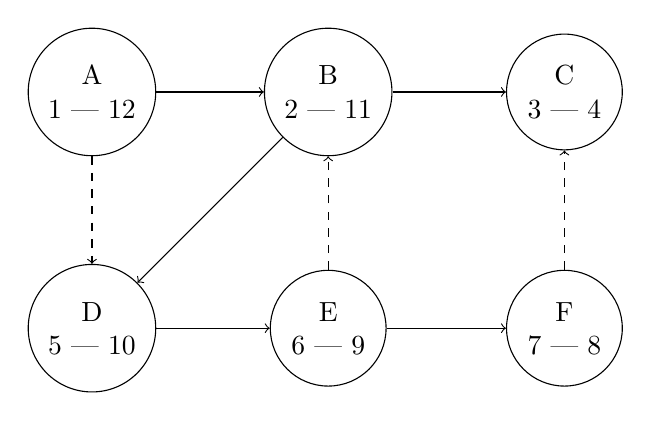
\begin{tikzpicture}[->, align=center]
\tikzstyle{v} = [circle, draw=black]
\tikzstyle{e} = [draw=black]
\tikzstyle{eh} = [draw=black, dashed]

\node[v](A) at (0, 3) {A\\1 | 12};
\node[v](B) at (3, 3) {B\\2 | 11};
\node[v](C) at (6, 3) {C\\3 | 4};
\node[v](D) at (0, 0) {D\\5 | 10};
\node[v](E) at (3, 0) {E\\6 | 9};
\node[v](F) at (6, 0) {F\\7 | 8};

\draw[e] (A) to (B);
\draw[e] (B) to (D);
\draw[eh] (A) to (D);
\draw[e] (D) to (E);
\draw[e] (E) to (F);
\draw[eh] (F) to (C);
\draw[e] (B) to (C);
\draw[eh] (E) to (B);
\end{tikzpicture}
\end{figure}
~\\
I figur \ref{fig:dfs} har vi brukt A som rotnode. Vi gikk deretter til et av barna, B. Videre gikk vi til C, og siden C har utgrad 0 måtte vi gå tilbake til B igjen. Fra B gikk vi videre til D, så til E og til F. Fra F går det en kant til C, men siden vi har besøkt C fra før går vi tilbake igjen. 

DFS-algorigmer er velegnet for å programmere rekursivt. Et eksempel på en enkel implementasjon i Java (som en metode i en Node-klasse):
\newpage
\javaimport{code/dfs.java}